\documentclass[tikz,border=2pt]{standalone}
\usepackage{amsmath,amssymb}
\usepackage{pgfplots}
\pgfplotsset{compat=1.18}

\begin{document}
% Jensen for convex g(x) = x^2 and a two-point X (0.2 or 1.4, equally likely): E[g(X)] is the
% midpoint of the chord, which lies above the curve value g(E X).
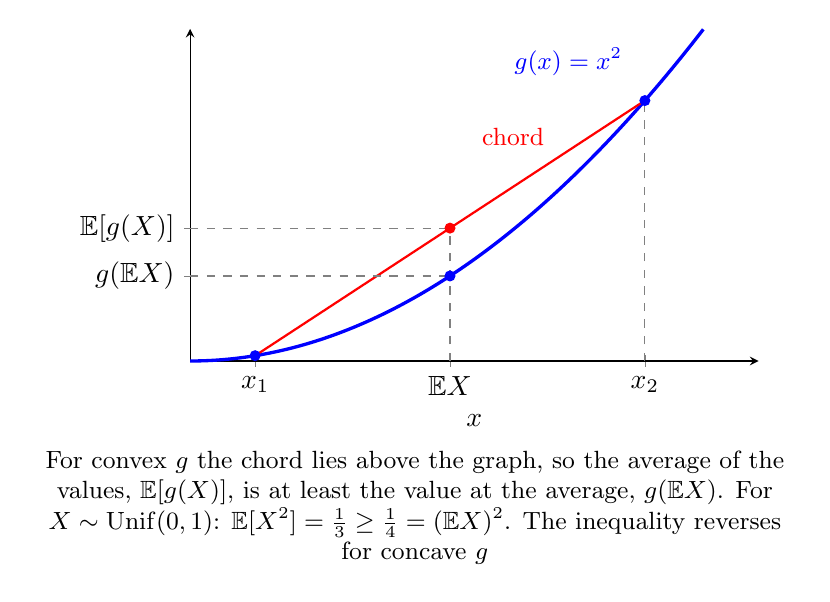
\begin{tikzpicture}
	\begin{axis}[
		axis lines=left, xmin=0, xmax=1.75, ymin=0, ymax=2.5,
		xtick={0.2,0.8,1.4}, xticklabels={$x_1$,$\mathbb{E}X$,$x_2$}, ytick={0.64,1.0}, yticklabels={$g(\mathbb{E}X)$,$\mathbb{E}[g(X)]$},
		xlabel={$x$},
		samples=100, smooth, width=8.8cm, height=5.8cm, clip=false
		]
		\addplot[blue, very thick, domain=0:1.58] {x^2};
		\draw[red, thick] (axis cs:0.2,0.04) -- (axis cs:1.4,1.96);
		\draw[gray, dashed] (axis cs:0.8,0) -- (axis cs:0.8,1.0);
		\draw[gray, dashed] (axis cs:0,1.0) -- (axis cs:0.8,1.0);
		\draw[gray, dashed] (axis cs:0,0.64) -- (axis cs:0.8,0.64);
		\draw[gray, dashed] (axis cs:0.2,0) -- (axis cs:0.2,0.04);
		\draw[gray, dashed] (axis cs:1.4,0) -- (axis cs:1.4,1.96);
		\fill[blue] (axis cs:0.2,0.04) circle (2pt);
		\fill[blue] (axis cs:1.4,1.96) circle (2pt);
		\fill[blue] (axis cs:0.8,0.64) circle (2pt);
		\fill[red] (axis cs:0.8,1.0) circle (2pt);
		\node[blue, anchor=east, font=\small] at (axis cs:1.36,2.25) {$g(x)=x^2$};
		\node[red, anchor=south east, font=\small] at (axis cs:1.12,1.55) {chord};
	\end{axis}
	\node[anchor=north, font=\small, align=flush center, text width=9.6cm] at ([yshift=-2pt]current axis.outer south) {For convex $g$ the chord lies above the graph, so the average of the values, $\mathbb{E}[g(X)]$, is at least the value at the average, $g(\mathbb{E}X)$. For $X\sim\operatorname{Unif}(0,1)$: $\mathbb{E}[X^2]=\tfrac13\ge\tfrac14=(\mathbb{E}X)^2$. The inequality reverses for concave $g$};
\end{tikzpicture}
\end{document}
